\chapter{Arrays and Linked Lists}

We will talk more about arrays in this chapter, with new concepts - linked lists, pointers and time complexity.

\section{Arrays in memory}

Let's go back to the example in Chapter 2.

\begin{lstlisting}
int x[8] = {3,1,4,1,5,9,2,6};
//alternatively: int x[] = {3,1,4,1,5,9,2,6}; length of array can be omitted as it can be derived from the right hand side

cout << x[0] << endl; //3 
cout << x[4] << endl; //5
cout << x[7] << endl; //6 (last element)
cout << x[8] << endl; //unexpected value 
\end{lstlisting}

The reason for x[8] to return an unexpected value rather than an error is pretty interesting. To understand that, you will need to know how arrays are stored, and how array elements are accessed. 

A \textbf{continuous} memory is allocated for each array. As indicated in the figure.

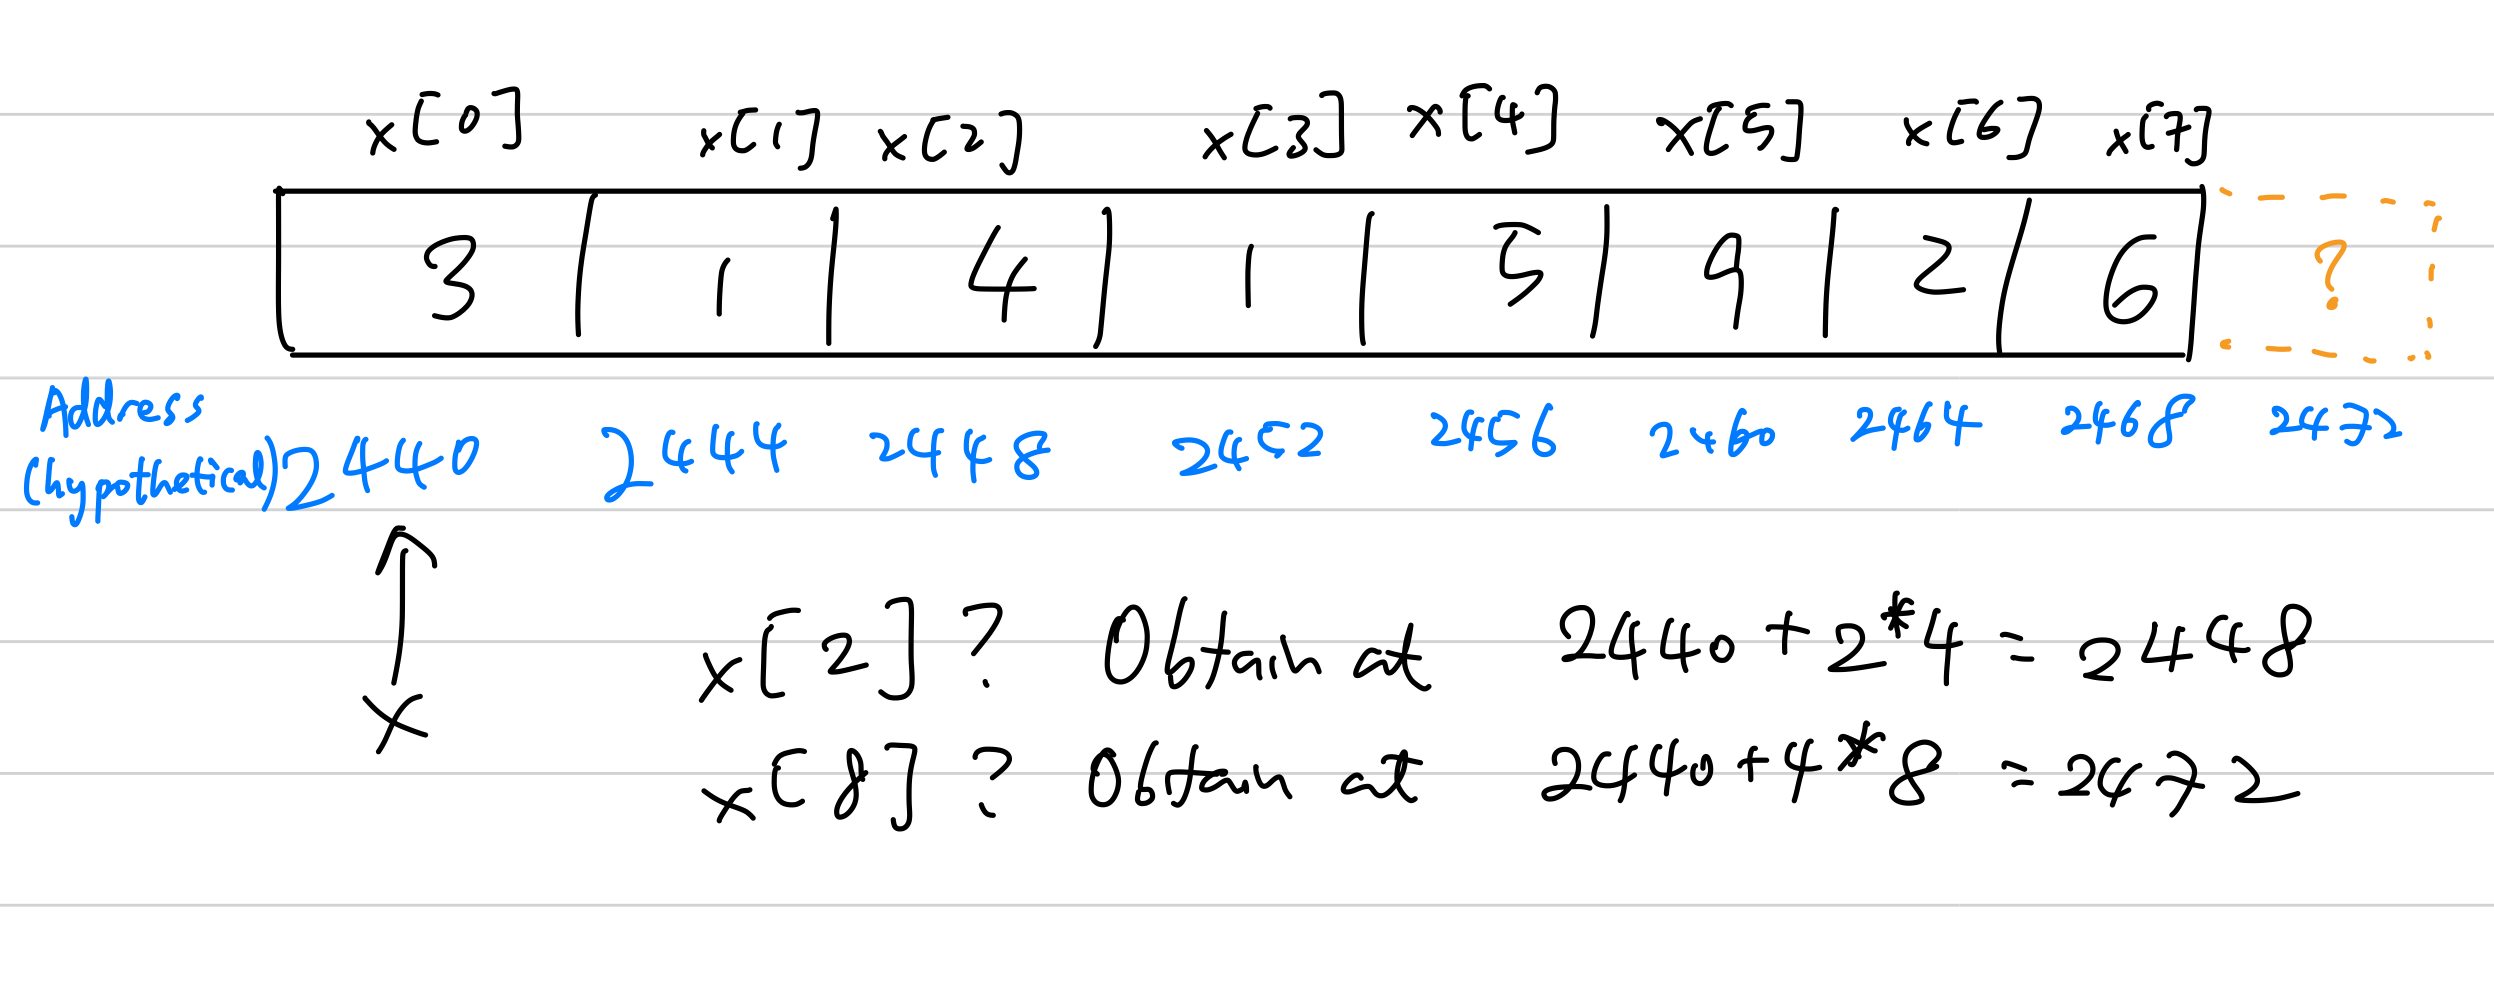
\includegraphics[width=13cm]{ch5-array.png}

C++ stores the base address of the array x, say at location 2240. Then to obtain x[k], it will calculate the address that it needs to retrieve by 2240 + k*4, the *4 is there because each integer occupies 4 bytes of memory, the multiplier is different depending on different datatypes. 

For example, when querying x[4], we obtained it from address 2240+16 = 2256. 

So, when querying x[8], we obtained it from address 2240+32 = 2272. What is in address 2272? We don't know! It is just a bunch of random 0s and 1s last modified by other programs. 
\vspace{6mm}

If you run this program multiple times, the result printed is different, this is because the base address of the array, allocated by the operating system and the C++ compiler, is different every time. 

Let's say, next time it ended up at base address 8084, then it will obtain x[8] at 8116, it probably stores a different sequence of 0s and 1s. While x[0..7] are the same, because that is what \texttt{int x[8] = {3,1,4,1,5,9,2,6};} does, put 3 at base address, put 1 at base address + 4, put 4 at base address + 8 ..., once the base address is allocated.

\section{Pointers}

Don't have time to cover, there should be plenty of resources online on this topic, including mycodeschool's playlist on pointers.

\section{Call by reference and call by value}

Testing testing

\section{Linked lists}

Scattered blocks of memory are allocated for the linked list. Each block of memory is called a \textbf{node}\index{node}. It contains a datum and also the reference to the next node. The only information we have is the reference to the first node, the \textbf{head}\index{head}. We will be able to read the whole list by \textbf{traversing}\index{traversing} the linked list, that is, to read the datum of the node and then proceed to another node by following the reference. Eventually if we reach a node with next = null, indicating that the end of the list is reached. As indicated in the figure.

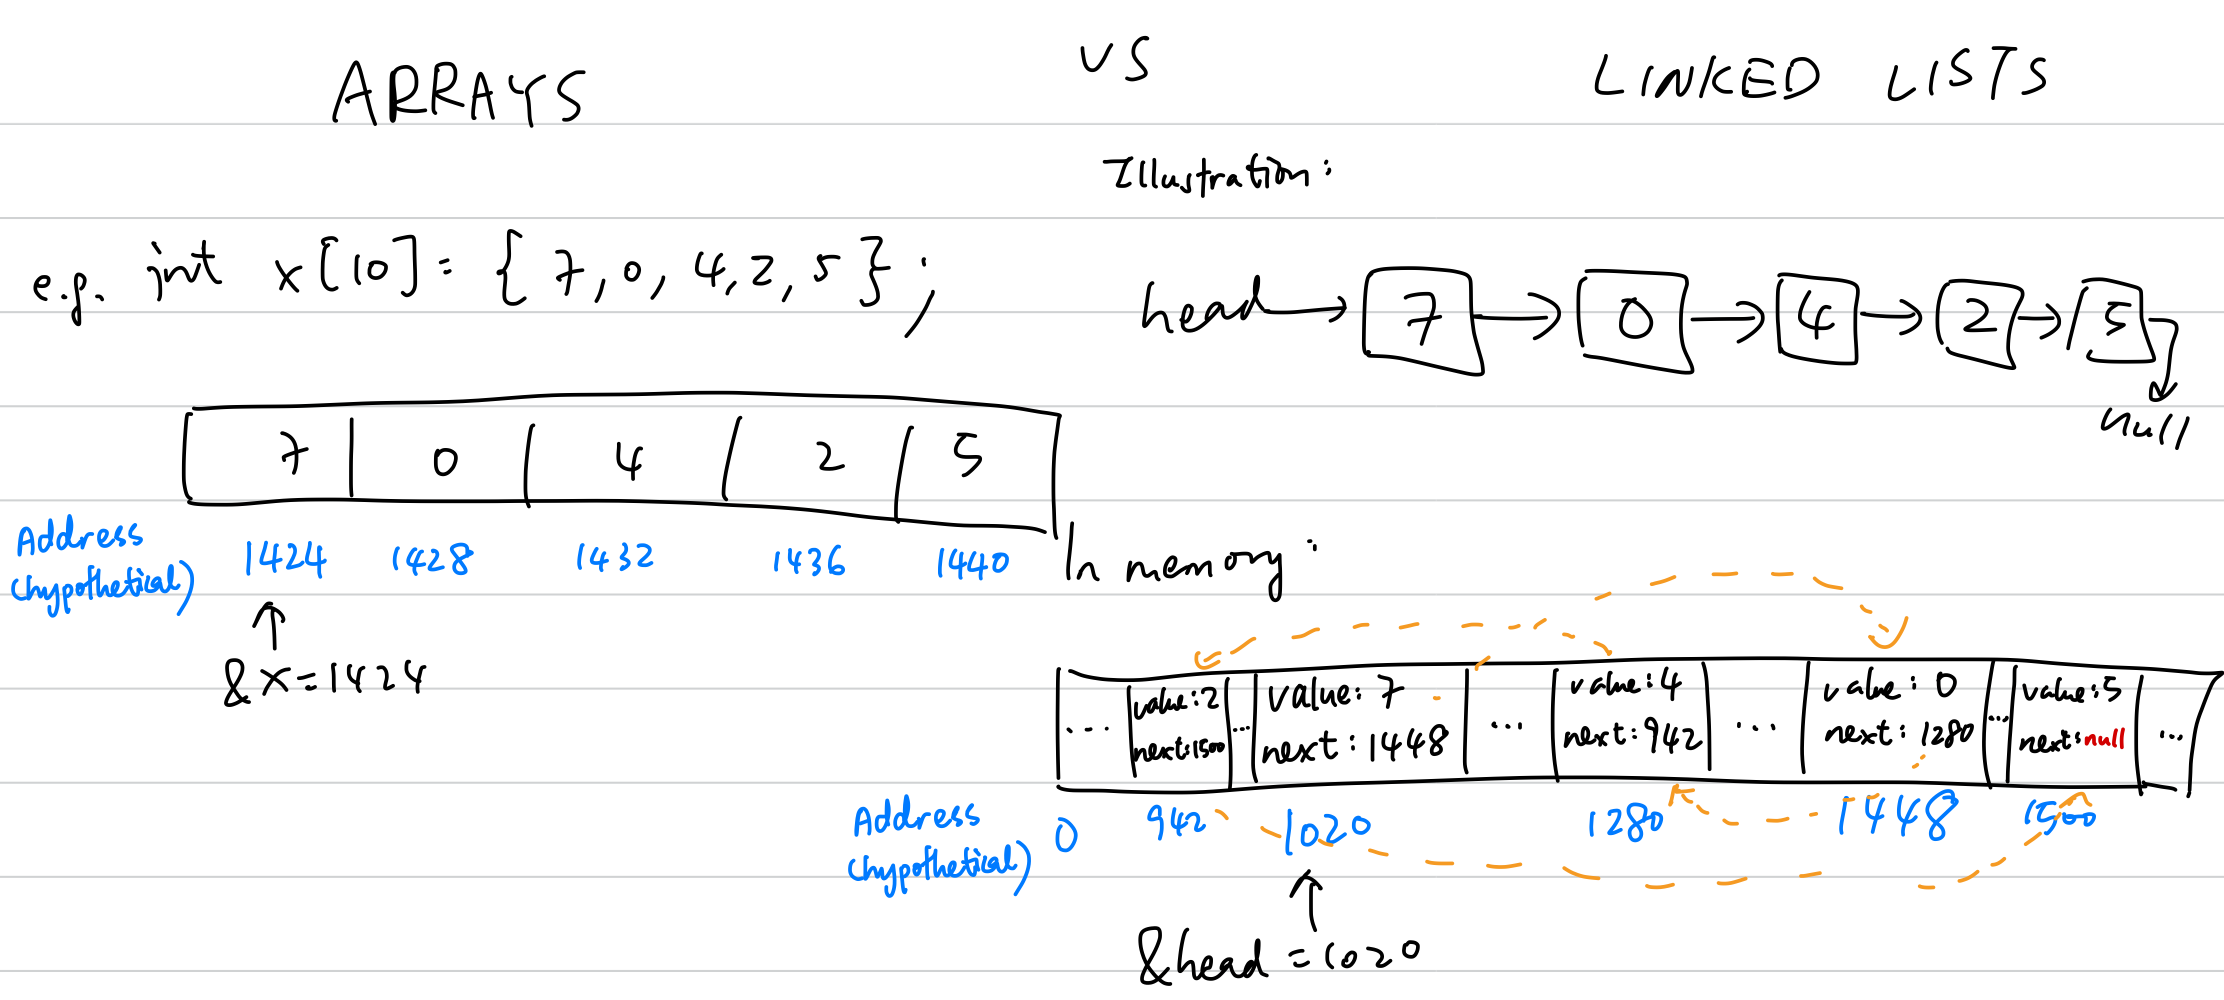
\includegraphics[width=15cm]{ch5-linkedlist1}

\section{Contrasting linked lists and arrays}

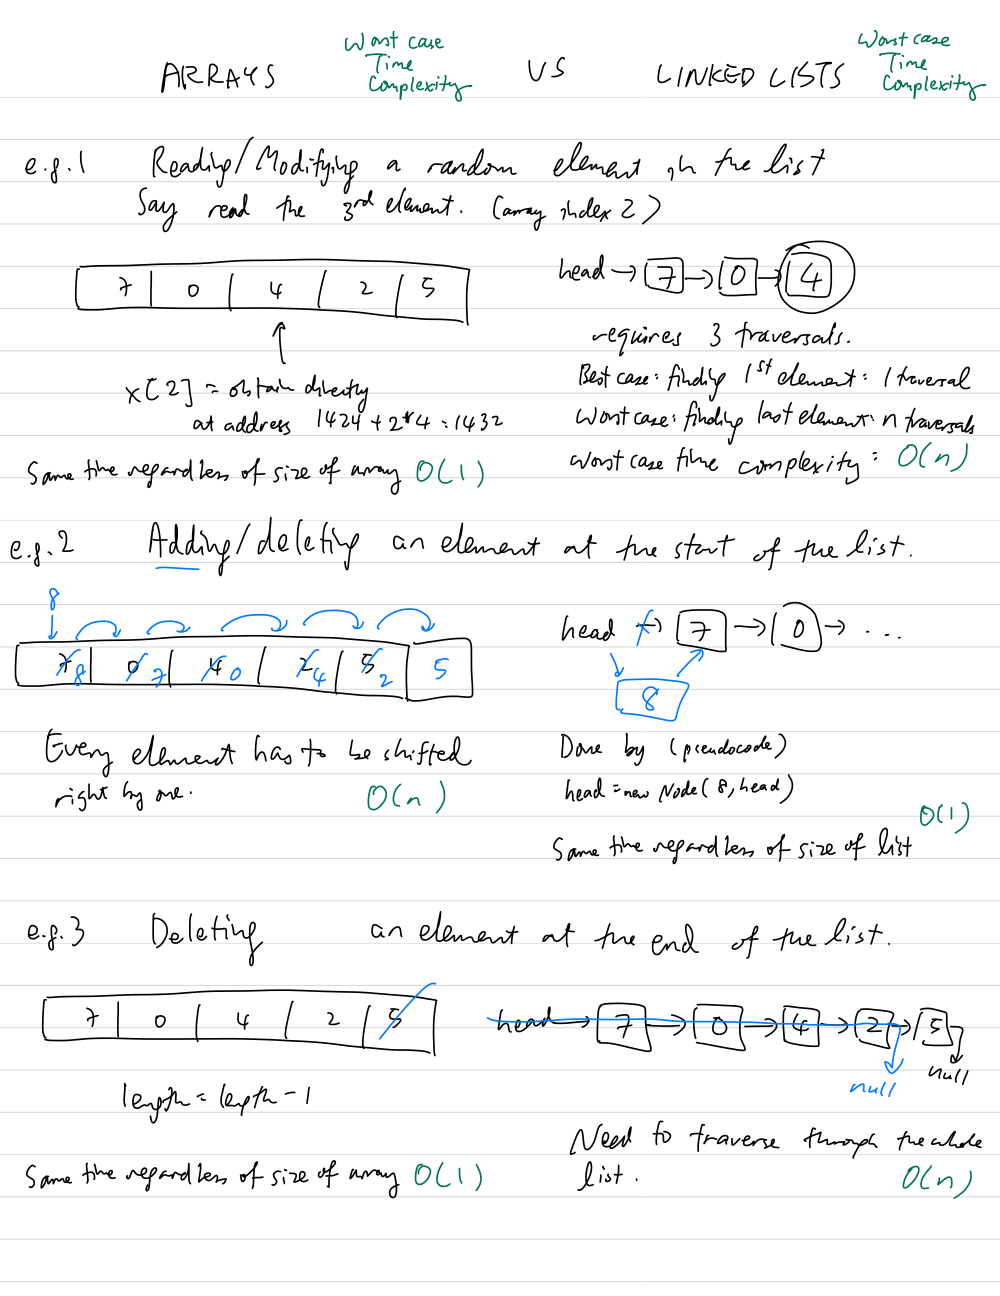
\includegraphics[width=15cm]{ch5-linkedlist2}

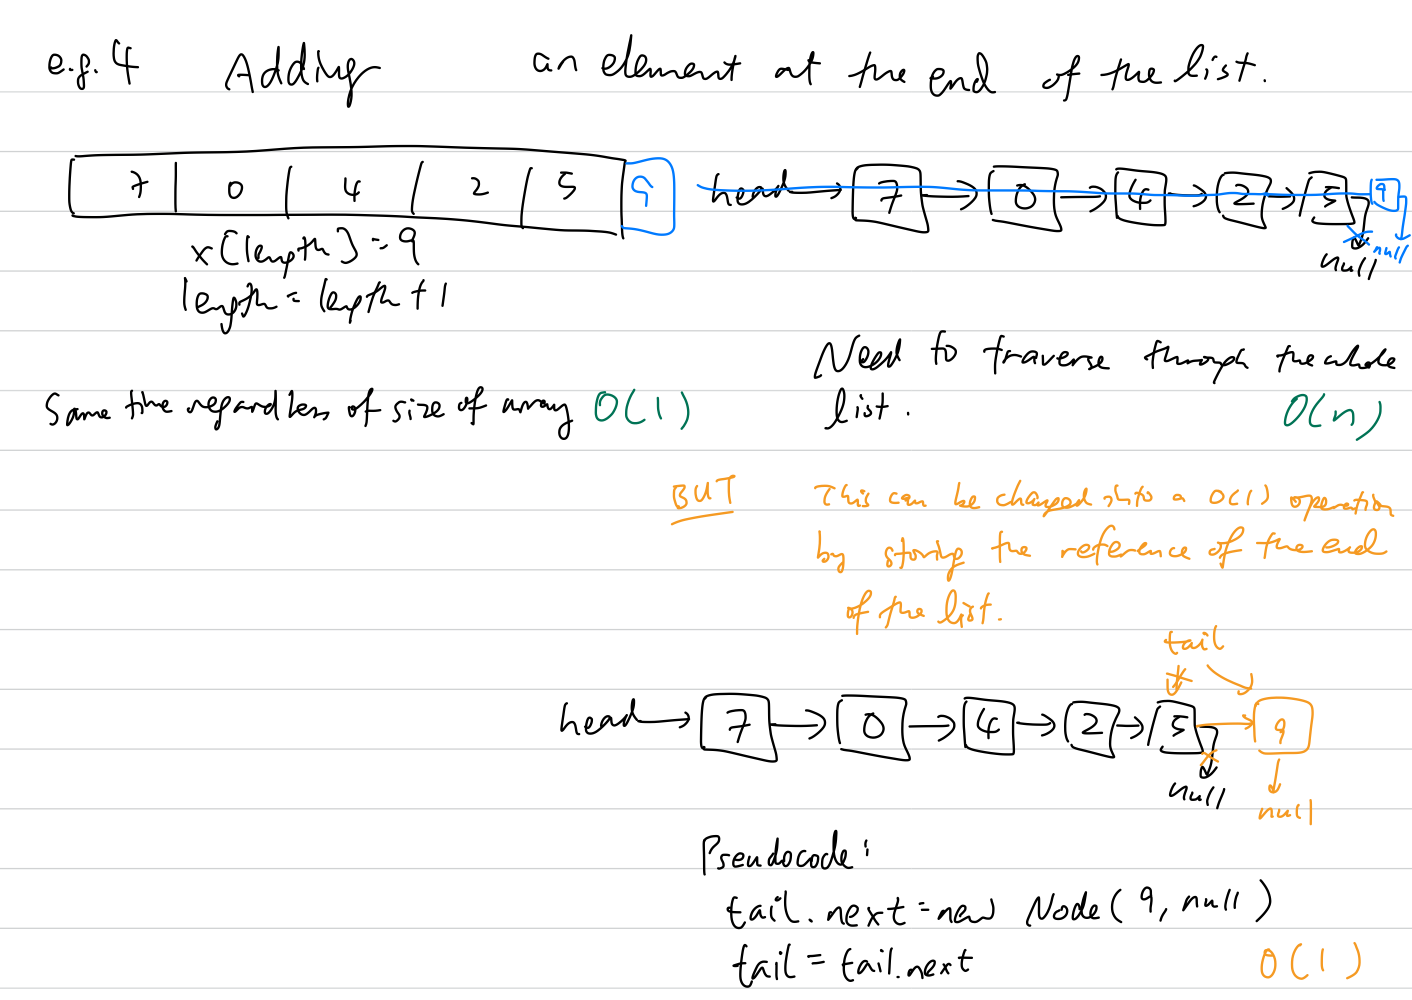
\includegraphics[width=15cm]{ch5-linkedlist3}

\section{Time complexity}



\section{Conclusion}
As you can see, linked lists and arrays have different efficiencies when performing different operations. There is no 'better' data structure, it is the job of we computer scientists to figure out which data structure should be used. Both linked lists and arrays can be used to implement stacks and queues and the algorithms that I will mention. 

Yet I do not advise you to code using linked lists in C++, because it is quite troublesome without automatic garbage collecting and with an inconvenient object-oriented programming infrastructure. It is best done using other languages like Java, Scala, or Python.

